\ifx\wholebook\relax\else
\input{../Common.tex}
\input{../macroes.tex}
\begin{document}
\fi


\chapter{Parameters and Arguments}\label{ch:argumenting}

\begin{chapterfigure}
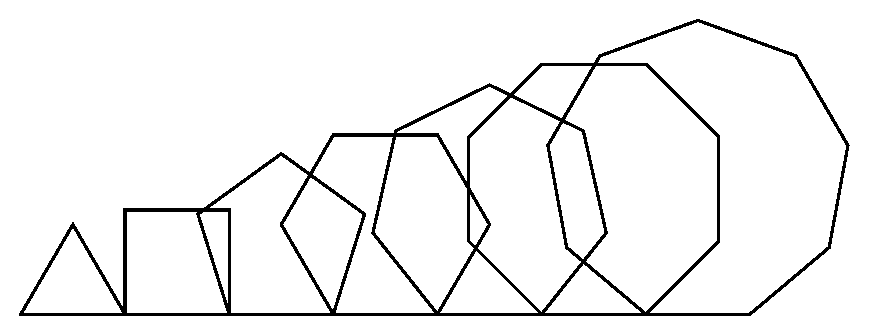
\includegraphics[width=0.9\linewidth]{ArgumentTitle}
\end{chapterfigure}

Up until now you sent messages with \emph{arguments}. For example, in the message \ct{go: 100} you specified that a robot should move a distance of 100 pixels and 100 is the argument of this message. You learned how to define methods but not how to define methods that require arguments. In this Chapter, you shall learn how to define methods whose behavior can be parameterized. Method parameters act as holes in the method definitions, holes that are filled when the message is sent.  First we will define a method with a parameter and invoke it, then we will analyze it.

%%%%%%%%%%%%%%%%%%%%%%%%%%%%%%%%%%%%%%%%%%%%%%%

\section{Parameter, you say?!}
The method \ct{square} defined in Chapter~\ref{mth:square} is
rather limited because the size of the square is fixed once for all. You certainly asked yourself what should be done to draw a square of 300 pixels or, 175, or 225 or even 23 pixels.  There is nothing preventing you to define the methods \ct{square300}, \ct{square175}, \ct{square225}, \ct{square23} and so on. But if we really look at it, creating multiple square methods does not solve the problem we have here. Because we do not want to define a new method each time. We would like to be able to specify the size of the square without having to define each time a new method!
For example, we would like to be able to draw squares whose size is given by a user and for that we do not want to define a method.

What we need is a kind of variable whose value will be assigned when the message will be sent and not before. This kind of variables exist in programming languages and are called \emph{parameter}. A method parameter is a special variable which can take any value we like \emph{at the moment the message is sent}, and not when we defined the method.

Come to think of it, this sounds familiar, doesn't it? After all, you know that methods such as \go or \turnLeft take a value (a distance or an angle) at the time the message is sent. All we have to do now is to understand how do we declare a method able to take arguments at execution time, just like the method \go.

\subsection{The method \ct{square:}}
We have seen that, in \st, the name of a method is terminated by a colon (\ct{:}) to indicate that the method requires an argument. Thus, if we want to create a method to draw a square with an arbitrary size, we will use \ct{square:} as name. We define the method \ct{square:} as shown in \methodref{mth:squareArguments}
This method is then invoked in the \scriptref{scr:usesquare}.

\begin{method}\label{mth:squareArguments}
square: \emph{size}
   "Draw a square of given size"

   4 timesRepeat: 
                    [ self go: \emph{size}.
                    self turnLeft: 90 ]
\end{method}

\begin{scriptwithtitle}{Using the method \ct{square:}}\label{scr:usesquare}
| \caro |
\caro := \Turtle new.
\caro square: 10.
\caro go: 300.
\caro square: 20
\end{scriptwithtitle}

Now let us analyze the method definition.  To define a method that requires one  argument, we terminated the method name with a colon \ct{:} and we wrote the name of the parameter, \eg \ct{size} in~\methodref{mth:squareArguments}. The parameter just represents a variable whose value is defined when the message is sent and not when the method is defined. In the script~\ref{scr:usesquare}, \ct{size} will take the value 10 during the first message \ct{square:\ 10} and then 20 during the message \ct{square:\ 20}.  The argument, however, does not need to be explicitly declared using vertical bars \ct{|} and \ct{|}.
 
In the method~\ref{mth:squareArguments} the name of the parameter is \ct{size}. The name of the parameter should represent what it is used for. Note that we could have named this parameter \ct{length} as in method~\ref{mth:squareArgumentslength}, or \ct{distance} as soon as we replace in the method body all the occurences of \ct{size} by \ct{length}. Note that  thes method~\ref{mth:squareArgumentslength} and  method~\ref{mth:squareArguments} are \emph{exactly} the same.

\begin{method}\label{mth:squareArgumentslength}
square: \emph{length}
   "Draw a square of given size"

   4 timesRepeat: 
                    [ self go: \emph{length}.
                    self turnLeft: 90]
\end{method}


\section{Practicing}
Now this is time to practice a bit. Let us start with a simple exercise.

\begin{exofigwithsizeandtitle}[0.5]{\includegraphics[width=6cm]{ArgHexagon}}{\ct{hexagon:}}
  Define the method \ct{hexagon:} that draws an hexagon with side of a given size.
\end{exofigwithsizeandtitle}

\begin{exofigwithsizeandtitle}[0.5]{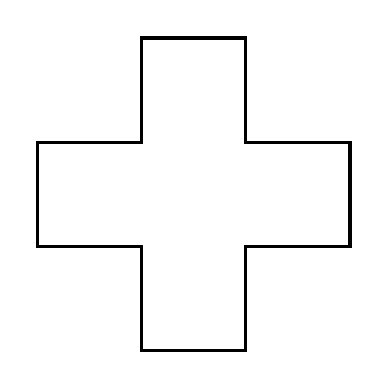
\includegraphics{Argcrossscr}}{Cross}
Transform the script given hereafter into a method named \ct{cross:} that draws a cross of a given size. You should then be able to execute the following expression: \ct{\caro\ cross:\ 100}. Hint: notice that 100/ 2 = 50.
\begin{nalltt}
|\caro|
\caro := \Turtle new.
4 timesRepeat: 
               [ \caro go: 50. 
               \caro turnLeft: 90. 
               \caro go: 100. 
               \caro turnRight: 90. 
               \caro go: 100.
               \caro turnRight: 90.
               \caro go: 50 ]

\end{nalltt}
\end{exofigwithsizeandtitle}


\largecadre{To define a method with multiple number of arguments terminate the words that compose the method name by a colon and place between them the parameters.\\
The method named \ct{polygon:size:} requires two arguments. The definition of the method \ct{polygon: sizeNumber size: size} defines two arguments \ct{sizeNumber} and \ct{size}.}

%%%%%%%%%%%%%%%%%%%%%%%%%%%%%%%%%%%%%%%%%%%%%%%
\section{Multiple Arguments}
Of course, it would be best to have a method drawing a polygon of given number of sides
\emph{and} size. The problem is how to create a method having two arguments?Creating a method with two arguments is obtained by writing a method name with two colons and placing the argument names after each colon.
Thus, in our case the method is called \ct{polygon:size:}. Its code is shown below. We can then simply send the message \ct{\caro\ polygon:\ 7\ size:\ 100}.

\begin{method}\label{mth:fixedSizePolygon}
polygon: sideNumber size: size
    "Draws a polygon of given number of sides and size"

    | angle length |
    angle := 360 / sideNumber.
    length := 4 * size / sideNumber.
    sideNumber timesRepeat: 
                               [ self go: length.
                               self turnLeft: angle ]
\end{method}



\paragraph{Implementation Remark.} You may wonder why we defined length as \ct{4 * size / sideNumber}. We decided to make the polygon' perimeter equals to the one of a
square having a side of size length. This way the perimeter is constant and all the polygons will be displayed using the same part of the screen. 

Here is the code of the method \ct{polygon100:} which draws a polygon of a given number of sides having a length of 100 pixels.

\begin{method}\label{mth:regularPolygon}
polygon100: sideNumber
    "Draws a polygon of given number of sides, the size of each
    side is 100 pixels"

    | angle |
    angle := 360 / sideNumber.
    sideNumber timesRepeat: 
                               [ self go: 100.
                               self turnLeft: angle ]
\end{method}

This method has one argument, \ct{sideNumber}, and one variable, \ct{angle}. Both of them are used within the code of the method. \ct{sideNumber} value is specified by a message that uses the method for example \ct{\caro\ polygon100:\ 7}, while the variable \ct{angle} is initialized by computing the angle corresponding to the parameter values (here 360 / 7). For each value of the \ct{sideNumber}, \ct{angle} will then take a specific value.

\begin{scriptfig}{Arghepta}{Using the method \ct{polygon100:}}\label{src:heptagon}
| \caro |
\caro := \Turtle new.
\caro polygon100: 7.
\end{scriptfig}

You may think that the name of the parameter \ct{sideNumber} is long. However, this name can easily be understood by any person reading the method. As we already discussed in Chapter~\ref{ch:furthervariables}, it is quite important that anyone be able read your code, almost like a novel. 



\begin{exonofig}
By slightly modifying the method \ct{cross:}, define the method
\ct{crossWidth:height:} that allows you to draw the picture shown in
Figure~\ref{fig:c8croix1}.  Note that a normal cross corresponds to
\ct{caro crossWidth: 30 height: 60}
\end{exonofig}


\begin{figure}[!h]
\begin{minipage}[c]{.3\linewidth}
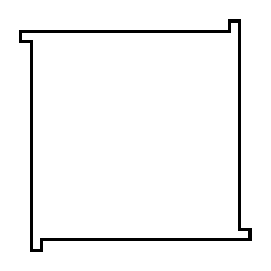
\includegraphics{Argcrossscr2.pdf}
\end{minipage}
\begin{minipage}[c]{.3\linewidth}
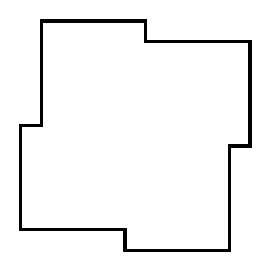
\includegraphics{Argcrossscr3}
\end{minipage}
\begin{minipage}[c]{.3\linewidth}

\includegraphics[width=5cm]{Argcrossscr4}
\end{minipage}
\label{c8croix1}
\caption{Three crosses produces respectively by : \ct{\caro crossWidth: 5 height: 50}, \ct{\caro crossWidth: 50 height: 5} and \ct{\caro crossWidth: 10 height: 20} \label{fig:c8croix1}}
\end{figure}




%%%%%%%%%%%%%%%%%%%%%%%%%%%%%%%%%%%%%%%%%%%%%%%
\section{Parameters and Variables}
Now that you practiced a bit, it is time to look a bit more carefully at the difference between variables and parameters. For this purpose let us compare the \scriptref{scr:Argsquarewithvariable} and the method \methodref{mth:squareArgumentsagain} defined earlier that we repeat here. 

From the \scriptref{scr:Argsquarewithvariable} we see that:  First the variable \ct{size} is declared (line 1), then we assign it a value (line 3) and then it is used as argument of the method \go (line 5).

\begin{scriptwithtitle}{The square script using a variable}\label{scr:Argsquarewithvariable}
(1)   | \caro \bold{size} | 
(2)   \caro := \Turtle new.
(3)   \bold{size := 10.}
(4)   4 timesRepeat: 
(5)               [ \caro go: \bold{size}.
(6)               \caro turnLeft: 90 ]
\end{scriptwithtitle}

Looking at \mthref{mth:squareArgumentsagain} we see that:
First the parameter \ct{size} is declared because it appears after
a colon in the method name (line 1). Second, it is used
as parameter of the message \go (line 5). A parameter does not have to be initialized because it always gets the value specified by the message that uses the method.

\begin{method}\label{mth:squareArgumentsagain}
(1) square: \bold{size}
(2)   "Draw a square of given size"
(3)
(4)   4 timesRepeat: 
(5)                    [ self go: \bold{size}.
(6)                    self turnLeft: 90]
\end{method}

\paragraph{Some Other Differences.}
Apart from the fact that a parameter is declared within the method's name, and not using variable declaration vertical bars \ct{||}, a parameter is used in the code of the method like any other variables. One difference that is specific to \st is that parameters are variables that cannot be modified. We cannot assign new values to parameters inside method bodies. The other difference is the way values are assigned to variables and parameters. A variable value is changed using \ct{:=}.  A parameter value is initialized when the method is executed. For example, \ct{\caro\ square:\ 10} initializes the parameter \ct{size} with the value \ct{10}. A parameter is a variable. However, the  parameter's value is only known when a message is sent and the method executed.

\begin{figure}[h]
\begin{center}
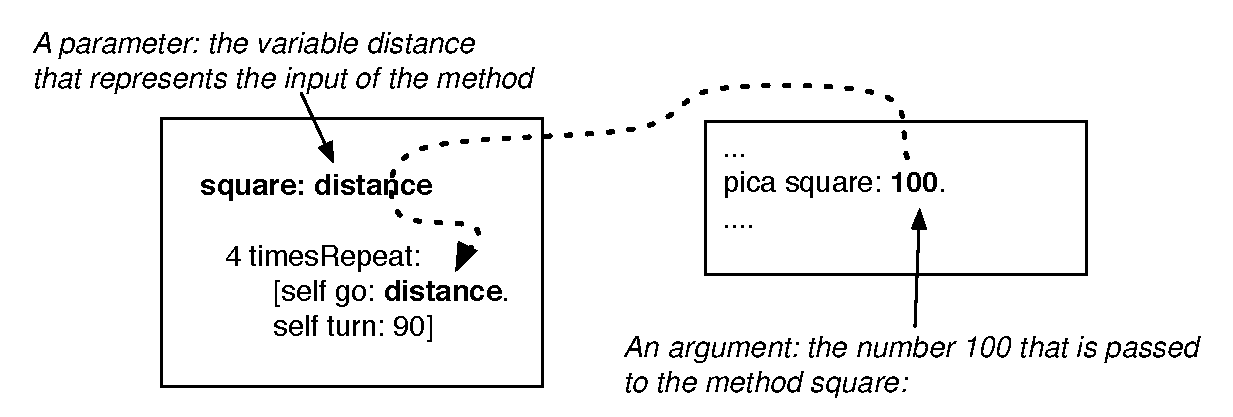
\includegraphics[width=10cm]{argparam2}
\caption{Difference between arguments (objects) and parameters (variables).\label{fig:argparam}}
\end{center}
\end{figure}

\section{Arguments and Parameters} 
We use the two terms \emph{arguments} and \emph{parameters}.  An argument is the actual object passed in a message, while a parameter is the variable used in the method definition\footnote{Other authors call argument actual parameters and parameters formal parameters, others use parameter and argument interchangeably.}. In Figure~\ref{fig:argparam}, in the message \ct{square: 100}, the number \ct{100} is the message argument. When the method \ct{square:} is executed its parameter \ct{distance} is initialized to \ct{100}, the value of the argument. Another way to understand the difference between an argument and a parameter is that a parameter a variable inside a method representing an input, while an argument is the actual value we pass to this input. Note that a parameter can also be used as an argument to other message sends. For example in the definition of the method \ct{square:} (method~\ref{mth:squareArguments}), the parameter \ct{size} is used as argument in the message \ct{go: size}.



A message argument can be also a variable. For example in \scrref{scr:varasArg}, the argument of the first message \ct{square:} is the value of the variable \ct{dist}, \ie 100. The argument of the second message \ct{square:} is the value of the expression \ct{dist + 200} \ie 300. The parameter \ct{size} of the method \ct{square:} will then takes the value \ct{100} for the first message and then the value \ct{300} for the last message send. 

\begin{scriptwithtitle}{A variable as argument}\label{scr:varasArg}
| \caro dist |
\caro := \Turtle new.
dist := 100. 
\caro square: dist.
\caro go: 300.
\caro square: dist + 200
\end{scriptwithtitle}

\begin{figure}[h]
\begin{center}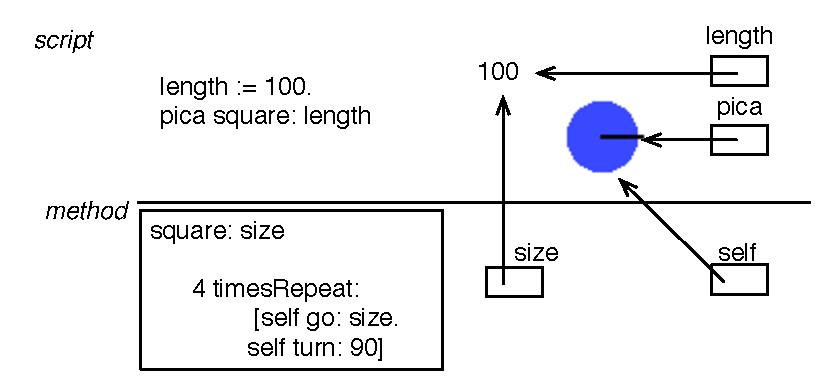
\includegraphics[width=8cm]{argumentBoxes}\end{center}
\caption{When a method is executed new variables are created that refer to the arguments and the receiver. \label{fig:argumentswithboxes}}
\end{figure}


\paragraph{About Method Execution.}
In fact when a method is executed new variables are created. These variables are the message receiver (\ct{self)}) and the parameters of the method that refer to the method argument (\ct{size}  in Figure~\ref{fig:argumentswithboxes}). Figure~\ref{fig:argumentswithboxes} shows the effect of sending the message \ct{square: length} to a robot referred by the variable \ct{pica}, the variable \ct{length} referencing the number \ct{100}. When the method \ct{square:} is executed, the variable \ct{self} refers to the message receiver, \ie the robot pointed to by the variable \ct{pica}, and the parameter \ct{size} refers to the value of the variable \ct{length}, \ie the number \ct{100}. 
The execution of the expression \ct{\daly\ square:\ 200} assigns to \self the robot referenced by the variable \daly and \ct{200} to the value of \ct{size}. 

This may look complex but you do not have to worry: Parameters are variables that are initialized with the values of the messages.



\summa

\begin{enumerate}
  \item A method parameter is declared right after the colon
  indicating the position of the parameter. It must not be declared as a  variable.
  
 \item To define a method with multiple number of arguments terminate the words that compose the method name by a colon and place between them the parameters.\\
The method named \ct{polygon:size:} requires two arguments. The definition of the method \ct{polygon: sizeNumber size: size} defines two arguments \ct{sizeNumber} and \ct{size}.\end{enumerate}



\ifx\wholebook\relax\else\end{document}\fi
